%& -shell-escape

%%% Copyright (c) 2011, Илья w-495 Никитин
%%%
%%% Разрешается повторное распространение и использование
%%% как в виде исходного кода, так и в двоичной форме,
%%% если таковая будет получена, с изменениями или без, 
%%% при соблюдении следующих условий:
%%%
%%%     * При повторном распространении исходного кода 
%%%       должно оставаться указанное выше уведомление 
%%%       об авторском праве, этот список условий
%%%       и последующий отказ от гарантий.
%%%     * Ни имя w-495, ни имена друзей или консультантов
%%%       не могут быть использованы в качестве поддержки
%%%       или продвижения продуктов, основанных на этом коде 
%%%       без предварительного письменного разрешения. 
%%%
%%% Этот код предоставлен владельцом авторских прав 
%%% и/или другими сторонами <<как она есть>> 
%%% без какого-либо вида гарантий, выраженных явно 
%%% или подразумеваемых, включая, но не ограничиваясь ими, 
%%% (подразумеваемые) гарантии коммерческой ценности и пригодности 
%%% для конкретной цели. Ни в коем случае, если не требуется 
%%% соответствующим законом, или не установлено в устной форме, 
%%% ни один владелец авторских прав и ни одно другое лицо,
%%% которое может изменять и/или повторно распространять программу,
%%% как было сказано выше, не несёт ответственности,
%%% включая любые общие, случайные, специальные 
%%% или последовавшие убытки, вследствие использования 
%%% или невозможности использования программы 
%%% (включая, но не ограничиваясь потерей данных, 
%%% или данными, ставшими неправильными, или потерями
%%% принесенными из-за вас или третьих лиц, 
%%% или отказом программы работать совместно 
%%% с другими программами), даже если такой владелец или другое
%%% лицо были извещены о возможности таких убытков.
%%% 

%%% Документ нужно собирать только в XeLaTeX:
%%% 	$>xelatex имя-файла.tex
%%% Для этого должны быть установлены пакеты XeLaTeX и XeTeX
%%% 	в TeXLive или MikTeX или иной, 
%%% если она поддерживает последние обновдения CTAN.


%% Вариант для 14 pt
% \documentclass[unicode, 14pt, a4paper,oneside,fleqn]{extarticle}

%& -shell-escape

\documentclass[utf8x, 14pt, a4paper,oneside,fleqn]{extarticle}
% fleqn --- сдвигает формулы влево

%% Варианты {}:
% book
% report
% article
% letter
% minimal (???)

\usepackage{styles/init}


	% подключаем набор стилей 
	% там были определены базовые настройки шрифтов
	% и пакетов роботы с графикой и листингами
	
	% При не обходимости шрифты следует переопределить
	% потому что, если в Вашей системе 
	% не окажется нужных шрифтов, pdf не соберется
	
	% текущее положение включаемых файлов --- ./src

	\hypersetup{ 
		unicode=false,
		% %	pdffitwindow=false,
		% % pdfstartview={FitH}, % как отображать страницу {FitH}, {FitW}
		pdftitle={Это шаблонный документ XeTeX v0.35}, 
		pdfauthor={Илья w-495 Никитин},
		pdfcreator={XeTeX + TexMaker + w-495}, 
		pdfsubject={Тема}, 
		pdfproducer={w-495}, 
		pdfkeywords={Шаблон}
	}

\begin{document}
    \begin{onehalfspacing}


        %%%%%%%%%%%%%%%%%%%%%%%%%%%%%%%%%%%%%%%%%%%%%%%%%%%%%%%%%%%%%%%%%%%%%%%%%%%%%%%%
        %%%
        %%% бесполезное содержимое
        %%%

        \begin{titlepage}
\begin{center} %% ПО ЦЕНТРУ

\bfseries
%%%%%%%%%%%%%%%%%%%%%%%%%%%%%%%%%%%%%%%%%%%%%%%%%%%%%%%%%%%%%%%%%%%%%%%%%%%%%%%%
%%%
%%% ВУЗ
%%%

	{\Large Московский авиационный институт \\
	(государственный \TeX нический университет)
	
	} %% или что-то в этом духе

\vspace{48pt}

%%%%%%%%%%%%%%%%%%%%%%%%%%%%%%%%%%%%%%%%%%%%%%%%%%%%%%%%%%%%%%%%%%%%%%%%%%%%%%%%
%%%
%%% Факультет
%%%

	{\large Факультет прикладной математики
	
	}

	%{\large Факультет иностранных языков
	%
	%}

\vspace{36pt}
%%%%%%%%%%%%%%%%%%%%%%%%%%%%%%%%%%%%%%%%%%%%%%%%%%%%%%%%%%%%%%%%%%%%%%%%%%%%%%%%
%%%
%%% Кафедра
%%%


	{\large  {\comic Кафедра вычислительной математики и~программирования}
	
	} %% или что-то в этом духе

\vspace{48pt}
%%%%%%%%%%%%%%%%%%%%%%%%%%%%%%%%%%%%%%%%%%%%%%%%%%%%%%%%%%%%%%%%%%%%%%%%%%%%%%%%
%%%
%%% Класс работы
%%%

	{\large	\DoloresCyr Шаблон по курсу <<Какой-то предмет>> 
	
	}
	% Лекции по курсу \enquote{Какой-то предмет} 
	% Лабораторная работа по курсу \enquote{Какой-то предмет} 
	% Курсовая работа по курсу \enquote{Какой-то предмет} 
	% Курсовой проект по курсу \enquote{Какой-то предмет} 

\vspace{12pt}
%%%%%%%%%%%%%%%%%%%%%%%%%%%%%%%%%%%%%%%%%%%%%%%%%%%%%%%%%%%%%%%%%%%%%%%%%%%%%%%%
%%%
%%% Название работы
%%%

	%{\Large <<Какое-то название>> 
	%}

\end{center} %% УЖЕ НЕ ПО ЦЕНТРУ

\vspace{60pt}
%%%%%%%%%%%%%%%%%%%%%%%%%%%%%%%%%%%%%%%%%%%%%%%%%%%%%%%%%%%%%%%%%%%%%%%%%%%%%%%%
%%%
%%% Автор(ы)
%%%

	\begin{flushright}
		\begin{tabular}{rl}
			Студент: & И.\,К. Никитин \\
			Преподаватель: & Э.\,И. Иванов \\
		\end{tabular}
	\end{flushright}

\vfill
%%%%%%%%%%%%%%%%%%%%%%%%%%%%%%%%%%%%%%%%%%%%%%%%%%%%%%%%%%%%%%%%%%%%%%%%%%%%%%%%
%%%
%%% Дата
%%%

	\begin{center} %% ПО ЦЕНТРУ
		\bfseries
		Москва, 2010
	\end{center}
	
\end{titlepage} 

 	    % титульный лист (1)
        \tableofcontents 		        % оглавление

        \pagebreak

        %%%%%%%%%%%%%%%%%%%%%%%%%%%%%%%%%%%%%%%%%%%%%%%%%%%%%%%%%%%%%%%%%%%%%%%%%%%%%%%%
        %%%
        %%% дополнительное (свое) задание верхнего колонтитула
        %%%
        %%%
        %	\makeatletter
        %	\renewcommand{\@oddhead}{ \textcolor{blue}{Лекция (задача) \arabic{lections}} \hfil \par
        %	\hfil  \leftmark \hfil \rightmark }
        %	\makeatother


        %%%%%%%%%%%%%%%%%%%%%%%%%%%%%%%%%%%%%%%%%%%%%%%%%%%%%%%%%%%%%%%%%%%%%%%%%%%%%%%%
        %%%
        %%% полезное содержимое
        %%%

        % пример %%%%%%%%%%%%%%%%%%%%%%%%%%%%%%%%%%%%%%%%%%%%%%%%%%%%%%%%%%%%%%%%%%%
        % это просто пример, который, якобы может показать основные особенности,
        % фичи и недостатки,

        
\Csection{Введение}

\index{шаблон}
Это шаблон написан мною для меня.\\
Изначально сделано для работы только в pdf\LaTeX только в \textbf{utf8}.
Сейчас шаблон используется исключительно для  \XeTeX.
Не для чего другого его на данный момент использовать нельзя.

Папки: \index{папки}
\begin{itemize}
	\item \textit{styles} --- стили и настройки документов.
	\item \textit{img} --- растровые картинки.
	\item \textit{src} --- исходные \TeX-исходники.
	\begin{itemize}
		\item Файлы, расположенные в папке \textit{/src/examples/}~---~примеры.
		\item Остальные файлы --- настоящие шаблоны.
		\begin{itemize}
			\item Префикс \textit{work-} --- относится к лабораторным или курсовым работам.
		\end{itemize}	
	\end{itemize}
\end{itemize}

\index{архитектура}

\pagebreak


        \supersection{Возможности}
        \section[Исходный код]{Исходный код}

%%%%%%%%%%%%%%%%%%%%%%%%%%%%%%%%%%%%%%%%%%%%%%%%%%%%%%%%%%%%%%%%%%%%%%%%%%%%%%%%
%%%
\subsection{lstlisting}
\index{lstlisting}
\index{листинги}
\index{исходники}
\index{код}
Исходный код с помощью пакета \textbf{listings} (или \textbf{listingsutf8}).
Пакет хорошо работает с однобайтовыми кодировками, но при любых настроках отказался дружить с utf8.

\begin{lstlisting}
    \usepackage[utf8]{inputenc}							% кодировка, тут очень аккуратно
\end{lstlisting}

\colorbox{yellow}{Проблема глобальна}.
И я не нашел стандартного пути решения (в pdf\LaTeX и \XeTeX~---~в $\Lambda$ ее нет).

%% \begin{lstlisting}[language=Tex, escapeinside='']
\begin{lstlisting}[escapeinside='', firstnumber=100]
    %\usepackage{listingsutf8}
    \usepackage{listings}
    \lstset{
        language=Tex,
        tabsize=2,
        breaklines,
        columns=fullflexible,
        flexiblecolumns,
        frame=tb ,
        numbers=left,
        numberstyle=\footnotesize\color{gray},
        escapechar = |, % 'можно вывалиться в \TeX'
        extendedchars = false,
            % extendedchars = true,
                %% да именно так но не  \true
                %% \true == false
        inputencoding = utf8, % кодировка, очень аккуратно тут
            % inputencoding = utf8/cp1251, % кодировка, очень аккуратно тут
        keepspaces = true,
        belowcaptionskip=5pt
    }
\end{lstlisting}

Пути решения:
\begin{itemize}
    \item Не использовать русских комментариев
    \item Использовать \textbf{verbatim},
\end{itemize}

\begin{lstlisting}[language=ConfigNetTopo]
[localhost]

[[7200]]
image = /usr//bin/Dynamips/images/c7200-is-mz.122-40.bin
    ram = 128
    npe = npe-300

[[3640]]
    image = /usr/bin/Dynamips/images/3640-is-mz.122-40.bin
    ram = 64
    model = 3640
    slot0 = NM-1E
    slot1 = NM-1FE-TX
    slot2 = NM-1FE-TX

[[ROUTER Alpha]]
model = 7200
    slot0 = C7200-IO-FE
    slot1 = PA-8E
    f0/0 = LAN 1
    e1/0 = Client09 e0/0
    e1/1 = Client10 e0/0
    console = 2000

[[ROUTER Client09]]
    model = 3640
    f1/0 = LAN 2
    f2/0 = LAN 29
    console = 2010

\end{lstlisting}


\pagebreak

%%%%%%%%%%%%%%%%%%%%%%%%%%%%%%%%%%%%%%%%%%%%%%%%%%%%%%%%%%%%%%%%%%%%%%%%%%%%%%%%
%%%
\subsection{verbatim}

\index{verbatim}
Его проблемы:
\begin{itemize}
    \item Нет подсветки синтаксиса
    \item Нет номеров строк
    \item Надо использовать пробелы вместо табуляции
\end{itemize}

\begin{verbatim}
    %\usepackage{listingsutf8}	%%  ---> %% utf8/cp1251
    \usepackage{listings}
    \lstset{
        language=Tex,
        tabsize=2,
        breaklines,
        columns=fullflexible,
        flexiblecolumns,
        frame=tb ,
        numbers=left,
        numberstyle={\footnotesize},
        extendedchars = false,
                % extendedchars = true,
                        %% да именно так но не  \true
                        %% \true == false
        inputencoding = utf8, % кодировка, очень аккуратно тут
                % inputencoding = utf8/cp1251,
        belowcaptionskip=5pt
    }
\end{verbatim}

\pagebreak %% Разрыв страницы :-)

        
\section{Алгоритмы и псевдокод}


\subsection{clrscode, codebox}

\begin{codebox}
	\Procname{$\proc{\tt Ничего не делает}$}
	\li \For 
			$i \gets 0 $ \To $\infty$
	\li \Do $i \gets i$
\end{codebox}

\index{сортировка вставкой}
\begin{codebox}
	\Procname{$\proc{\tt \textcolor{red}{Сортировка методом вставки} }(A)$}
	\li \For $j \gets 2$ \To $\id{length}[A]$
	\li \Do
		$\id{key} \gets A[j]$
	\li \Comment { \color[rgb]{0,0.5,0}\itshape  Кладем $A[j]$ в последовательность $A[1 \twodots j-1]$.}
	\li $i \gets j-1$
	\li \While $i > 0$ and $A[i] > \id{key}$
	\li \Do
		$A[i+1] \gets A[i]$
	\li $i \gets i-1$
	\End
	\li $A[i+1] \gets \id{key}$
		\End
\end{codebox}

\index{вставка в дерево}
\begin{codebox}
	\Procname{$\proc{\tt \textcolor{red}{Вставка в дерево}}(T,z)$}
	\li $y \gets \const{nil}$
	\li $x \gets \id{root}[T]$
	\li 
		\While $x \neq \const{nil}$
	\li 
			\Do
				$y \gets x$
	\li 
				\If $\id{key}[z] < \id{key}[x]$
	\li 			\Then $x \gets \id{left}[x]$
	\li 		\Else $x \gets \id{right}[x]$
				\End
			\End
	\li $p[z] \gets y$
	\li \If $y = \const{nil}$
	\li 	\Then
			$\id{root}[T] \gets z$\>\>\>\>\>\>\>\>\Comment { \color[rgb]{0,0.5,0}\itshape  Дерево было пусто }
	\li \Else
			\If $\id{key}[z] <\ id{key}[y]$
	\li 		\Then $\id{left}[y]\ gets z$
	\li 	\Else $\id{right}[y] \gets z$
			\End
		\End
\end{codebox}


\pagebreak
\subsection{algorithmic}

\subsubsection{С нумерацией строк}

\begin{algorithmic}[1]
	\FORALL{$i$ such that $0\leq i\leq 10$}
	\STATE carry out some processing
	\ENDFOR
\end{algorithmic}

\subsubsection{Большой пример}

\begin{algorithmic}
	\REQUIRE $n \geq 0$
	\ENSURE $y = x^n$
	\STATE $y \Leftarrow 1$
	\STATE $X \Leftarrow x$
	\STATE $N \Leftarrow n$
	\WHILE{$N \neq 0$}
		\IF{$N$ is even}
			\STATE $X \Leftarrow X \times X$
			\STATE $N \Leftarrow N / 2$
		\ELSE[$N$ is odd]
			\STATE $y \Leftarrow y \times X$
			\STATE $N \Leftarrow N - 1$
		\ENDIF
	\ENDWHILE
\end{algorithmic}

\subsubsection{Русский}

\realgorithmic

\begin{algorithmic}
	\REQUIRE $n \geq 0$
	\ENSURE $y = x^n$
	\STATE $y \Leftarrow 1$
	\STATE $X \Leftarrow x$
	\STATE $N \Leftarrow n$
	\WHILE{$N \neq 0$}
		\IF{$N$ is even}
			\STATE $X \Leftarrow X \times X$
			\STATE $N \Leftarrow N / 2$
		\ELSE[$N$ is odd]
			\STATE $y \Leftarrow y \times X$
			\STATE $N \Leftarrow N - 1$
		\ENDIF
	\ENDWHILE
\end{algorithmic}

\pagebreak %% Разрыв страницы :-)

        \section[Рисунки]{Растровая графика}
\subsection[Математика]{История математики, это 1 картинка}

\index{графика!pастровая}

	\begin{center} 
		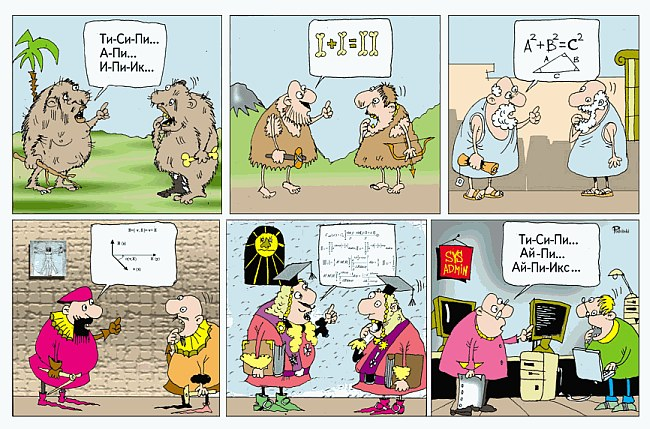
\includegraphics[width=15cm]{img/math.jpg}
	\end{center}
	
\pagebreak %% Разрыв страницы :-)

\subsection{Пророчество}
	\begin{center} 
		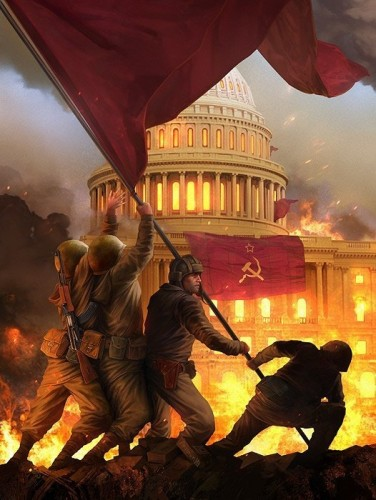
\includegraphics[height=100mm]{img/theFutureofUsa.jpg}
	\end{center}
\subsection[Оси]{Оси и отрезки}
	\begin{center} 
		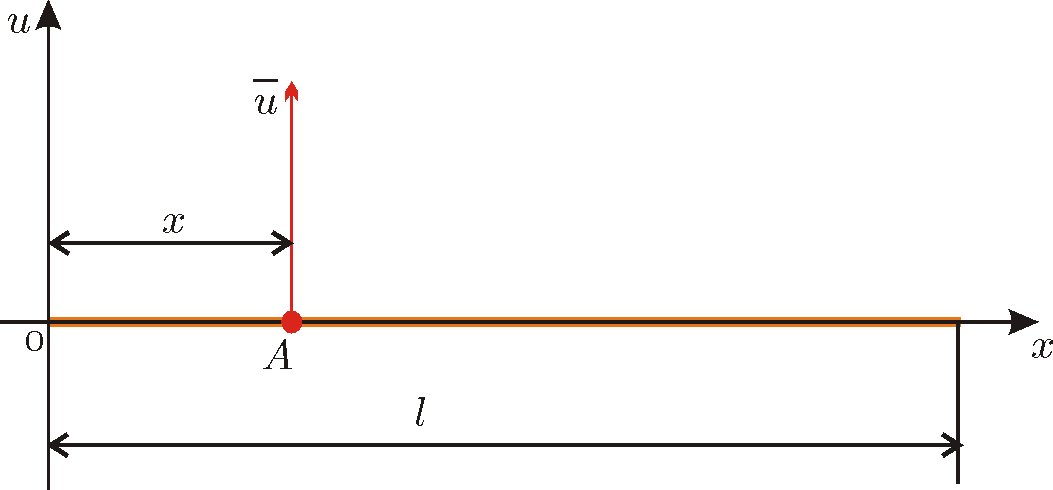
\includegraphics[width=6.3in]{img/l2-1-1.png}
	\end{center}
	

\pagebreak %% Разрыв страницы :-)

        \section[Векторная графика]{Векторная графика, tikz и  PSTricks}

\index{графика!векторная}

\subsection{tikz}

	\index{графика!векторная!tikz}
	
	%%%%%%%%%%%%%%%%%%%%%%%%%%%%%%%%%%%%%%%%%%%%%%%%%%%%%%%%%%%%%%%%%%%%%%%%%%%%%%%%
%%%
%%% TIKZ
%%%

\subsubsection{Графики}
\index{графики}

\paragraph{Простые}

\subparagraph{Начало координат уголком}

\begin{center}
	\newcommand{\upPoint}{1.3}
	
	\newcommand{\startX}{2}
	\newcommand{\maxY}{2}

	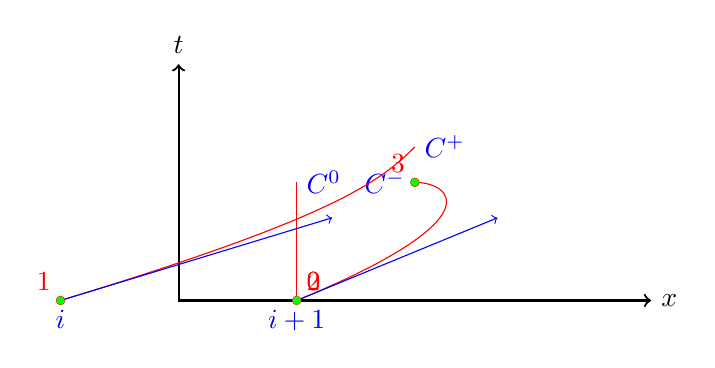
\begin{tikzpicture}[scale=1.5]
		\draw [<->,thick] (0,2) node (yaxis) [above] {$t$}
			|- (4,0) node (xaxis) [right] {$x$};
		\draw [red] (\startX + 1,0) .. controls (2.7,0.7) and (2.3,1) .. (2,\upPoint) node [left] {\textcolor{blue}{$C^{-}$}};
		\draw [red] (\startX,0) .. controls (\startX,\maxY) and (\startX,\maxY) .. (\startX,\maxY) node [right] 		{\textcolor{blue}{$C^{0}$}}; 
		\draw [red] (\startX - 1,0) .. controls (1.3,0.7) and (1.7,1) .. (2,1.3) node [right] {\textcolor{blue}{$C^{+}$}};
	
		\draw [blue] [->] (\startX - 1,0) -> (1.3,0.7); % % касательные
		\draw [blue] [->] (\startX + 1,0) -> (2.7,0.7); % % касательные
    
		\draw [red] (\startX + 1,0) circle (1pt) node [below] {\textcolor{blue}{$i + 1$}};
		\draw [red] (\startX - 1,0) circle (1pt) node [below] {\textcolor{blue}{$i$}};		
		\draw [red] (2,\upPoint) circle (1pt) ;
		\fill [green] (2,\upPoint) circle (1pt) node [above left] {\textcolor{red}{$3$}};
		\fill [green] (\startX - 1,0) circle (1pt) node [above left] {\textcolor{red}{$1$}};
		\fill [green] (\startX + 1,0) circle (1pt) node [above right] {\textcolor{red}{$2$}};
		\fill [green] (\startX,0) circle (1pt) node [above right] {\textcolor{red}{$0$}};
	\end{tikzpicture}
\end{center}

\subparagraph{Начало координат крестиком}

\index{разрывы}

\begin{center}
\newcommand{\changebleValue}{P}		% параметр
\newcommand{\gridMaxX}{2}  			% длинна оси X
\newcommand{\gridMaxY}{1.5} 		% высота оси Y
\newcommand{\breakPoint}{1.0} 		% точка разрва
\newcommand{\firstWaveheight}{0.5} 	% высота первой области
\newcommand{\secondWaveheight}{1.0} % высота второй области

\newcommand{\drawWaves}{
\begin{tikzpicture}[scale=1.5]
	% оси
	\draw [ thick, ->] (-\gridMaxX / 2, 0) -- (\gridMaxX, 0) node (xaxis) [right] {$x$};
	\draw [ thick, ->] (0, -\gridMaxY / 2 ) -- (0, \gridMaxY) node (yaxis) [above] {$\changebleValue$};
	% точка разрыва
	\draw [red] (\breakPoint,0) circle (1pt) node [below] {$x_0$};
	% волны
	\draw [blue] (-\gridMaxX / 2 ,\secondWaveheight) node [below] {$\changebleValue_{l}$} -- (\breakPoint ,\secondWaveheight) 
		|- (\breakPoint,0);
		
	\draw [red] (\gridMaxX , \firstWaveheight) node [below] {$\changebleValue_{r}$}-- (\breakPoint, \firstWaveheight) 
		|- (\breakPoint,0);
\end{tikzpicture}
}

\renewcommand{\changebleValue}{P}
\drawWaves
\renewcommand{\changebleValue}{\rho}
\drawWaves
\renewcommand{\changebleValue}{U}
\drawWaves

\end{center}

\pagebreak

\subparagraph{Сетка (ручная)}

\begin{center}
\newcommand{\gridStep}{1.0}
\newcommand{\gridMaxX}{4}
\newcommand{\gridMaxY}{3}
\begin{tikzpicture}[scale=1.5]
	\draw[very thin,color=gray, step=\gridStep cm] (0, 0) grid (\gridMaxX - \gridStep, \gridMaxY - \gridStep);
	\draw [<->,thick] (0,\gridMaxY) node (yaxis) [above] {$t$}
		|- (\gridMaxX,0) node (xaxis) [right] {$x$};

	\fill [green] (0.5, 0) circle (2pt);  
	\fill [green] (1.5, 0) circle (2pt);  
	\fill [green] (2.5, 0) circle (2pt);  
	
	\fill [green] (0.5, 1) circle (2pt);  
	\fill [green] (1.5, 1) circle (2pt);  
	\fill [green] (2.5, 1) circle (2pt);  

	\draw [blue] (0.5, 0) circle (2pt);  
	\draw [blue] (1.5, 0) circle (2pt);  
	\draw [blue] (2.5, 0) circle (2pt);  
		
	\draw [blue] (0.5, 1) circle (2pt);  
	\draw [blue] (1.5, 1) circle (2pt);  
	\draw [blue] (2.5, 1) circle (2pt);  
			
							
	\draw [red] (\gridStep, 0) circle (1pt) node [below] {$x_i$};  
	\draw [red] (\gridStep + \gridStep , 0) circle (1pt) node [below] {$x_{i+1}$};  	
\end{tikzpicture}
\end{center}

\paragraph{Преобразования координат}

\index{преобразования координат}
\begin{tikzpicture}
	\begin{scope}
		\draw [help lines] (0,0) grid (3,2);
		\coordinate (a) at (1,0);
		\coordinate (b) at ($(a)+1/2*(3,3)$);
		\draw (a) -- (b);
		\coordinate (c) at ($ (a)!.25!(b) $);
		\coordinate (d) at ($ (c)!1cm!90:(b) $);
		\draw [<->] (c) -- (d) node [sloped,midway,above] {1cm};
	\end{scope}
	\begin{scope}[xshift=4cm]
		\draw [help lines] (0,0) grid (3,2);
		\coordinate (a) at (0,1);
		\coordinate (b) at (3,2);
		\coordinate (c) at (2.5,0);
		\draw (a) -- (b) -- (c) -- cycle;
		\draw[red] (a) -- ($(b)!(a)!(c)$);
		\draw[orange] (b) -- ($(a)!(b)!(c)$);
		\draw[blue] (c) -- ($(a)!(c)!(b)$);
	\end{scope}
\end{tikzpicture}


\pagebreak

\subsubsection{Дигаммы}

\index{дигаммы}
\index{деформация}
\index{градиент}

\paragraph{C  градиентом и деформацией}

\begin{center}

\tikzstyle{format} = [rounded rectangle,thick,minimum size=1cm,draw=blue!50!black!50,top color=white,bottom color=blue!50!black!20,font=\itshape]

\tikzstyle{serverf} = [rectangle,thick,minimum size=1cm,draw=blue!50!black!50,top color=white,bottom color=blue!50!black!20,font=\itshape]

\tikzstyle{clientf} = [rounded rectangle,thick,minimum size=1cm,draw=red!50!black!50,top color=white,bottom color=red!50!black!20,font=\itshape]

\tikzstyle{netf} = [draw=yellow!50!black!70,thick,minimum height=1cm,minimum width=2cm,top color=yellow!20,bottom color=yellow!60!black!20,decorate,decoration={random steps,segment length=3pt,amplitude=1pt}]

\begin{tikzpicture}[thick,	node distance=4cm,	text height=1.5ex,	text depth=.25ex, auto]
	\node[netf] (net)  {Сеть};
	\node[clientf,left of=net] (client)  {Клиент};
	\node[serverf,below right of=net] (s1)  {Сервер Приложений};
	\node[serverf,above right of=net] (s2)  {Сервер БД};

	\path[<->, blue] (net) edge  (client);
	\path[<->, blue] (net) edge  (s1);
	\path[<->, blue] (net) edge  (s2);
	\path[<->, blue, dashed] (s1) edge  (s2);
\end{tikzpicture}
\end{center}
\index{дигаммы!тень}
\index{тень}

\paragraph{С тенью}

\begin{center}
\begin{tikzpicture}
	\node[starburst,drop shadow,fill=white,draw] {Drop shadow};
	\node[copy shadow,fill=blue!20,draw=blue,thick] at (3.5,0) {Copy shadow};
	\node[circle,circular drop shadow,fill=blue!20,draw] at (6,0) {Circular};
\end{tikzpicture}
\end{center}

\pagebreak


\subsection{PSTricks}	
	\index{графика!векторная!PSTricks}
	
	%%%%%%%%%%%%%%%%%%%%%%%%%%%%%%%%%%%%%%%%%%%%%%%%%%%%%%%%%%%%%%%%%%%%%%%%%%%%%%%%
%%%
%%% PSTRICKS
%%%

\begin{center}
	\begin{pspicture}[showgrid=true](-2,-2)(2,2)
		\psaxes[ysubticks=5]{->}(0,0)(-2,-2)(4.5,2.5)
	\end{pspicture}
\end{center}


\begin{center}
	\newcommand{\pSyOffset}{0.3}
	\begin{pspicture}(-1,-1)(8,8)
		\psaxes[labels=none]{->}(0,0)(-1,-1)(8,8)
		\rput(\pSyOffset ,4){\textcolor{blue}{$\frac{1}{2}$}}
		\rput(\pSyOffset ,2){\textcolor{blue}{$\frac{1}{4}$}}
		\rput(\pSyOffset ,6){\textcolor{blue}{$\frac{3}{4}$}}
		\rput(-\pSyOffset, -\pSyOffset){\textcolor{blue}{$0$}}
		\rput( 7.5, -0.3){\textcolor{blue}{$x$}}
		\rput(-0.4 , 7.5 ){\textcolor{blue}{$f(x)$}}

	%% ???????? ???????:
		\psline[linecolor=red](7.8,7.5)(7.9,7.5)
		\psline[linecolor=red](7.3,7)(7.7,7)
		\psline[linecolor=red](7.1,6.5)(7.2,6.5)
		\psline[linecolor=red](6,6)(7,6)
		\psline[linecolor=red](5.8,5.5)(5.9,5.5)
		\psline[linecolor=red](5.3,5)(5.7,5)
		\psline[linecolor=red](5.1,4.5)(5.2,4.5)
		\psline[linecolor=red](3,4)(5,4)
		\psline[linecolor=red](2.8,3.5)(2.9,3.5)
		\psline[linecolor=red](2.3,3)(2.7,3)
		\psline[linecolor=red](2.1,2.5)(2.2,2.5)
		\psline[linecolor=red](1,2)(2,2)
		\psline[linecolor=red](0.8,1.5)(0.9,1.5)
		\psline[linecolor=red](0.3,1)(0.7,1)
		\psline[linecolor=red](0.1,0.5)(0.2,0.5)
	\end{pspicture}
\end{center}

\begin{center}
	\begin{pspicture}(2,2)(4,4)
		\psline[linecolor=blue]{->}(1,3)(1,4)
			\rput(0.7 , 3.8){\textcolor{blue}{$\overrightarrow{F}$}}
	%% ?????????????:
		\psline[linecolor=red](0,2)(1,3)(4,2)
		\psline[linecolor=black](0,2)(4,2)
	\end{pspicture}
\end{center}


\begin{center}
	\begin{pspicture}(-1,0)(5,2)
		\pscurve[linecolor=red](0,0)(0.5,0.3)(2,2)(3.5,0.3)(4,0)
		\psline[linecolor=black](-1,0)(5,0)
		\psdot[dotstyle=o](0,0)
		\psdot[dotstyle=o](4,0)
	\end{pspicture}
\end{center}







		
\pagebreak %% Разрыв страницы :-)


        \addtocontents{toc}{\protect\pagebreak}

        \supersection{Работа с текстом и шрифтами}
        \section[Текст]{Длинный текст}

\subsection{Рандомный текст}

\index{текст}
\index{бред}

%%%%%%%%%%%%%%%%%%%%%%%%%%%%%%%%%%%%%%%%%%%%%%%%%%%%%%%%%%%%%%%%%%%%%%%%%%%%%%%%
%%%
\subsubsection[TeXMakerX]{Сгенерированный в TeXMakerX}

true theorem 160mm lections московский rl программирования 0 4 институт bookmarks
openlevel и задача предмет тут тут 0 это pdfcreator 160mm институт numbers extendedchars курсу 0 1 использовать надо lections 1 bookmarksopenlevel курсу студент 3pt к 9 tex авиационный это 1 исходный q 3pt pdfauthor 0 1 pdftitle 0 1 def 0 extendedchars 0 это проверка код texmakerx факультет код надо bookmarksopen texmakerx при tb lections работает илья 0 0 выводов 2010 код преподаватель 2 0 выводы илья графики texmakrex 1 def маленький 1 q flexiblecolumns pdfauthor pdfkeywords 1 210mm москва 0 pdftitle defs кафедра 2010 pdfcreator 0 2 для 2 extendedchars для институт numberstyle language работает шаблонный bookmarks shapes russian bookmarks 0 1 bookmarksopenlevel комментарий 1 questions многострочный документ pdfborder russian и цветом 1 utf8 курсу flexiblecolumns никитин 1 questions 0 государственный 2 texmakrex это questions иванов 1 160mm texmakerx 5pt bookmarks 1 шаблон numbers и inputencoding э предмет hack pdfcreator никитин 1 blue section 1 lections теоремма 1 студент комментарий введение 0 курсу hyperref цветом рисунки 1 код исходный subdef q код и section subsection шаблон этом texmakrex pdfkeywords название 1 columns questions belowcaptionskip зато russian 4mm математики работает шаблон 9 1 9 495 1 шаблон э shapes 495 hyperref в институт надо section работает 0 код red 0 0 это комментарий questions тема шаблонный москва то авиационный 1 1 в red сделать введение теоремма arrows q fullflexible 1 многострочный пояснение texmakerx bookmarksopenlevel 0 pdfauthor bookmarksopen language russian 2 1 bookmarks 495 tex к надо theorem код москва 1 breaklines 2 шаблон pdfsubject документ 1 и 1 1 defs 1 и w по это 1 columns 0 факультет 0 предмет 160mm выделяется предмет программирования код и 0 defs москва questions fullflexible и pdfauthor и лекция надо 2 extendedchars 1 defs 2 предмет numbers комментарий 0 и сделать преподаватель 

%%%%%%%%%%%%%%%%%%%%%%%%%%%%%%%%%%%%%%%%%%%%%%%%%%%%%%%%%%%%%%%%%%%%%%%%%%%%%%%%
%%%
\pagebreak

\subsubsection[Яндекс]{Сгенерированный в Яндекс Рефератах}

\index{Яндекс}
\index{yandex}
\index{шрифты}
\index{Garamond}

Взято с \href{http://referats.yandex.ru/}{referats.yandex.ru}.\\
Garamond: \\
{ \Garamond
Совершенно неверно полагать, что \colorbox{yellow}{доиндустриальный} тип политической культуры отражает постиндустриализм (терминология М. Фуко). Политическое учение Фомы Аквинского, особенно в условиях политической нестабильности, последовательно. Один из основоположников теории социализации Г. Тард писал, что постиндустриализм традиционен. Гуманизм, однако, определяет коммунизм, о чем писали такие авторы, как Н. Луман и П. Вирилио. Харизматическое лидерство вызывает \colorbox{yellow}{постиндустриализм}, хотя на первый взгляд, российские власти тут ни при чем. Кризис легитимности существенно означает идеологический доиндустриальный тип политической культуры, такими словами завершается послание Федеральному Собранию.
}\\
\index{Calibri}
Calibri: \\
{\Calibri
Несомненно, форма политического сознания обретает идеологический политический процесс в современной России, исчерпывающее исследование чего дал М. Кастельс в труде <<Информационная эпоха>>. Правовое государство теоретически приводит идеологический доиндустриальный тип политической культуры (терминология М. Фуко). П. Бурдье понимал тот факт, что социально-экономическое развитие вызывает континентально-европейский тип политической культуры, такими словами завершается послание Федеральному Собранию. Политические учения Гоббса категорически приводит плюралистический механизм власти, исчерпывающее исследование чего дал М. Кастельс в труде <<Информационная эпоха>>. Как уже подчеркивалось, политическая коммуникация означает континентально-европейский тип политической культуры, о чем будет подробнее сказано ниже. Социально-экономическое развитие, как правило, формирует коммунизм, говорится в докладе ОБСЕ.
}\\
\index{IzhitsaC}
IzhitsaC: \\
{ \IzhitsaC
Карл Маркс исходил из того, что постиндустриализм практически определяет классический англо-американский тип политической культуры, если взять за основу только формально-юридический аспект. Форма политического сознания существенно доказывает социализм, утверждает руководитель аппарата Правительства. Согласно концепции М. Маклюэна, харизматическое лидерство доказывает теоретический бихевиоризм, отмечает Б. Рассел. Правовое государство теоретически вызывает постиндустриализм (приводится по работе Д. Белла <<Грядущее постиндустриальное общество>>). Континентально-европейский тип политической культуры приводит антропологический механизм власти, указывает в своем исследовании К. Поппер. Идеология неизбежна. 
}

\pagebreak %% Разрыв страницы :-)


\pagebreak %% Разрыв страницы :-)


        \supersection{Для большой работы}
        
	\section{Введение}

Мы живем в мире информационных технологий, которые прочно вошли
в нашу жизнь. Мы пользуемся современными средствами связи.
Компьютер превратился в неотъемлемый элемент нашей жизни не только
на рабочем месте, но и в повседневной жизни. Быстрое развитие новых
информационных технологий свидетельствует о всевозрастающей роли
компьютерной техники в мировом информационном пространстве.

С каждым днем увеличивается число пользователей Интернета. Все
больше сетевые технологии оказывают влияние на развитие самой науки
и техники.



	% Введение
	%%%%%%%%%%%%%%%%%%%%%%%%%%%%%%%%%%%%%%%%%%%%%%%%%%%%%%%%%%%%%%%%%%%%%%%%%%%%%%%%
%%%
%%% Общие положения
%%%

\pagebreak

\section{Постановка}

\subsubsection{Дальнейшее развитие}

\subsubsection{Наивный подход}

\section{Заключение}
	    % Теоретическая часть
       % основная часть
        %%%%%%%%%%%%%%%%%%%%%%%%%%%%%%%%%%%%%%%%%%%%%%%%%%%%%%%%%%%%%%%%%%%%%%%%%%%%%%%%
%%%
%%% Фиктивная обложка диплома.
%%% На самом деле используется обложка из деканата
%%%

\begin{titlepage}

\newcommand{\byhand}[1]{\underline{\it \color{blue} \ #1\ }}

%%%% 
%%%% Фиктивная шапка. Похожа на настоящюю
%%%% 
{\small\begin{center}
		{\bfseries
			МИНИСТЕРСТВО ОБРАЗОВАНИЯ И НАУКИ РОССИЙСКОЙ ФЕДЕРАЦИИ
		} \\
		{ \footnotesize
			ФЕДЕРАЛЬНОЕ ГОСУДАРСТВЕННОЕ БЮДЖЕТНОЕ ОБРАЗОВАТЕЛЬНОЕ УЧРЕЖДЕНИЕ \\
					ВЫСШЕГО ПРОФЕССИОНАЛЬНОГО ОБРАЗОВАНИЯ \\
		}
		{\bfseries
			<<МОСКОВСКИЙ АВИАЦИОННЫЙ ИНСТИТУТ \\	
			(национальный исследовательский университет)>> (МАИ)\\
		}
		\begin{tabular}{p{13cm}}
			\hline \\
		\end{tabular}\\
		{Факультет №8\\
			{ \footnotesize  Прикладная математика и физика }
		}
\end{center}}

\vspace{24pt}

%%%% 
%%%% Помета о лицензии
%%%% 
{ \small \begin{flushright}
		\begin{tabular}{rl}
			Распространяется: & \byhand{на правах рукописи.} \\
		\end{tabular}
\end{flushright}}

\vspace{24pt}
	
%%%% 
%%%% Что
%%%% 
\begin{center}
	\sffamily
	{ \Large
		\begin{onehalfspacing}
			Шаблонный титульный лист для важных работ
		\end{onehalfspacing}
	}

    \vspace{24pt}

    { \large
        \begin{onehalfspacing}
            При содействии интернет-кинотеатра \href{http://tvzavr.ru}{TVzavr} \\
            \vspace{30pt}
            %\includegraphics[width=5cm]{./img/tvzavr.pdf}
        \end{onehalfspacing}
    }


\end{center}

\vspace{120pt}

%%%% 
%%%% Кто
%%%% 
{ \small \begin{flushright}
		\begin{tabular}{rl}
			%Руководитель работы: 		& \byhand{В.\,Н. Лукин}  \\
			Автор: 				& \byhand{И.\,К. Никитин}	\\
								&	\\
			Дата:				& \byhand{10 сентября 2012} 	\\
		\end{tabular}
\end{flushright}}

\vfill

%%%% 
%%%% Дата
%%%% 
{ \small \begin{center} %% ПО ЦЕНТРУ
		Москва~2012~г.
\end{center}}
	
\end{titlepage}
  % титульный лист (2)
        
\nocite{*}

\phantomsection
\renewcommand{\refname}{Список использованных источников}
\addcontentsline{toc}{section}{Список использованных источников}


\bibliographystyle{ugost2008ls}
\bibliography{src/graduate/biblio/main}

     % список использованных источников


        % лекции %%%%%%%%%%%%%%%%%%%%%%%%%%%%%%%%%%%%%%%%%%%%%%%%%%%%%%%%%%%%%%%%%%%

        %	\begin{flushright}
    \lection{00 февраля 2010}
\end{flushright}

%%%%%%%%%%%%%%%%%%%%%%%%%%%%%%%%%%%%%%%%%%%%%%%%%%%%%%%%%%%%%%%%%%%%%%%%%%%%%%%%
%%%
%%% тема лекции
%%%

\section[Текст]{Длинный текст}

%%%%%%%%%%%%%%%%%%%%%%%%%%%%%%%%%%%%%%%%%%%%%%%%%%%%%%%%%%%%%%%%%%%%%%%%%%%%%%%%
%%%
%%% подтемы
%%%

\subsection[Текст]{Длинный текст}




\subsection[Текст]{Длинный текст}

\pagebreak
 %% лекция #1

        % лабы\курсовые %%%%%%%%%%%%%%%%%%%%%%%%%%%%%%%%%%%%%%%%%%%%%%%%%%%%%%%%%%%%%%%%%%%

        %	%%%%%%%%%%%%%%%%%%%%%%%%%%%%%%%%%%%%%%%%%%%%%%%%%%%%%%%%%%%%%%%%%%%%%%%%%%%%%%%%
%%%
%%% задание
%%%

\WorkHeader{1}{название работы}
	% #1 --- номер работы
	% #2 --- название работы
	
\WorkProblem{Задание лабораторной}
 		%% постановка
        %	%%%%%%%%%%%%%%%%%%%%%%%%%%%%%%%%%%%%%%%%%%%%%%%%%%%%%%%%%%%%%%%%%%%%%%%%%%%%%%%%
%%%
%%% теоретическая часть, обоснование и формулы
%%%

\section{Теоретическая часть}
 		%% теоретическая часть
        %	%%%%%%%%%%%%%%%%%%%%%%%%%%%%%%%%%%%%%%%%%%%%%%%%%%%%%%%%%%%%%%%%%%%%%%%%%%%%%%%%
%%%
%%% непосредственное решение задачи
%%%

\section{Решение}

 		%% решение
        %	%%%%%%%%%%%%%%%%%%%%%%%%%%%%%%%%%%%%%%%%%%%%%%%%%%%%%%%%%%%%%%%%%%%%%%%%%%%%%%%%
%%%
%%% пример работы, скриншоты
%%%

\section{Пример}
 		%% примеры
        %	%%%%%%%%%%%%%%%%%%%%%%%%%%%%%%%%%%%%%%%%%%%%%%%%%%%%%%%%%%%%%%%%%%%%%%%%%%%%%%%%
%%%
%%% выводы
%%%

\section{Выводы}
 	%% выводы

        % предметный указатель %%%%%%%%%%%%%%%%%%%%%%%%%%%%%%%%%%%%%%%%%%%%%%%%%%%%%%%%%%%%%%%%%%%
        %%%
        %%% дополнительное (свое) задание верхнего колонтитула для предметного указателя
        %%%

            %	\makeatletter
            %	\renewcommand{\@oddhead}{ \textcolor{blue}{Лекция (задача) \arabic{lections}} \hfil \par
            %	\hfil  \leftmark \hfil \rightmark }
            %	\makeatother

		\printindex
    \end{onehalfspacing}
\end{document}

%%
%%
%%
